\documentclass[12pt,floatnumber=continuous,espaco=umemeio]{abnt}

\usepackage{ist-modelo-2}
\usepackage[section]{placeins}

\section{PHP}

\acs{PHP} é uma linguagem de programação interpretada simples e poderosa,
projetada para criar conteúdo \acs{HTML}. Sendo que esta tecnologia pode ser
utilizada: em linha de comando, em aplicações \ac{GUI} utilizando uma biblioteca
chamada \acs{PHP-GTK} e principalmente em servidores web para gerar conteúdo
dinâmico \cite{programmingPhp}.

Sendo assim, o \acs{PHP} é um projeto \textit{open source} (de código aberto),
portanto, em outras palavras, significa que você tem acesso ao código-fonte e
pode utilizar, alterar e redistribuir tudo sem custos \cite{phpAndMysqlWebDevelopment}.

\subsection{As Versões do PHP}

A linguagem de programação \acs{PHP} surgiu em 1994, sendo que, foi criada por
Rasmus Lerdorf para o acompanhamento de visitas em seu currículo online, nesta
época foi batizada de \textit{Personal Home Page Tools}, sendo esta
frequentemente chamada apenas de \textit{PHP Tools}, no entanto, esta primeira
versão da tecnologia tratava-se apenas de um conjunto de binários \ac{CGI},
porém, em 1995 o criador da linguagem adicionou novas funcionalidades ao projeto
e o rebatizou de \ac{PHP/FI} \cite{phpProgramandoComOrientacaoAObjetos}.

Enquanto que, a segunda versão foi lançada em 1996, onde, 
Rasmus reescreveu a versão inicial e a chamou de \acs{PHP/FI} 2.0, que incluia 
suporte aos seguintes bancos de dados: \textit{mSQL},
\textit{Postgres98} e \textit{DBM} \cite{programmingPhp}.

Entretanto, devido a problemas de instabilidade Andi Gutmans e Zeev
Suraski (fundadores da \acs{Zend}, \textbf{Ze}ev + A\textbf{nd}i) e Rasmus, em
1997 iniciaram outra reescrita da linguagem, sendo que, em 1998 foi lançada a versão
que mais se assemelha com o \acs{PHP} dos dias atuais, a versão 3, que deixou
de lado o nome \acs{PHP/FI} e passou a adotar a nomenclatura \ac{PHP}
\cite{websitePHPHistoria}.

Segundo \citeonline{phpProgramandoComOrientacaoAObjetos}, logo após o lançamento
da versão 3, Zeev e Andi passaram a trabalhar na reescrita do núcleo da 
linguagem afim de melhorar a sua performance, sendo assim, rebatizaram o
\textit{core} dando-lhe o nome de \textit{Zend Engine}, por conseguinte, em
2000 foi lançado o \acs{PHP} 4, que incluiu uma grande melhoria de desempenho, 
além do suporte a: sessões, vários bancos de dados e vários servidores web.

Quatro anos depois, em 2004 surge a versão 5 da linguagem \acs{PHP}, que incluí
um novo \textit{core} a \textit{Zend Engine} 2.0, incluindo dentre as principais
melhorias, o suporte à programação orientada a objetos já existente
em outras linguagens, tais como: \textit{Java} e \textit{C++}
\cite{phpProgramandoComOrientacaoAObjetos}.

Você poderá realizar o \textit{download} de qualquer uma das versão citadas
acima acessando o museu da linguagem \cite{websitePHPMuseum}.

\begin{document}

	% Título do Projeto
\renewcommand{\title}{Desenvolvimento de um Sistema Web de Simulado para a ZCPE}

% Nome do autor
\author{João Paulo Cercal}

% Localização
\newcommand{\ano}{2014}
\newcommand{\cidade}{Joinville}
\newcommand{\semestre}{1}

% Informações da instituição de ensino
\newcommand{\faculdade}{CENTRO UNIVERSITÁRIO TUPY – UNISOCIESC}
\newcommand{\universidade}{SOCIEDADE EDUCACIONAL DE SANTA CATARINA – SOCIESC}
\newcommand{\curso}{Sistemas de Informação}

% Orientador
\orientador{Prof. Msc. Leila Regina Techio}

% Palavras chave
\newcommand{\ptBRKeyword}{Lorem. Ipsum. Consectetur.} 
\newcommand{\enUSKeyword}{Lorem. Ipsum. Consectetur.}

% Frase da folha de rosto
 \newcommand{\fraseFolhaRosto}{Este trabalho foi apresentado ao Centro Universitário Tupy - UNISOCIESC como
pré-requisito para a obtenção de grau de bacharel em \curso.}

%\newcommand{\orientacao}{ Orientador: \ABNTorientadordata. \\ Co-orientador: \ABNTcoorientadordata.}
\newcommand{\orientacao}{ Orientador: \ABNTorientadordata.}

% Frase de aprovação
\newcommand{\fraseAprovacao}{Trabalho de Dissertação sob o título \title, apresentado por \authoraprovacao, e aprovado em \ABNTdatadata, em \ABNTlocaldata, pela banca examinadora constituída conforme abaixo:}

% Frase de dedicatória
\newcommand{\fraseDedicatoria}{Dedico este trabalho aos meus pais, Sebastião Techio e Inez Anita Ely Techio (\textit{in memorian}) pelo exemplo de dignidade, dedicação e amor. A minha filha Nathalia, pela paciência, amor e compreensão.}

% Frase de agradecimento
\newcommand{\fraseAgradecimento}{A Deus que possibilitou que este trabalho fosse finalizado.
				Ao professor Dr. Mehran Misaghi por acreditar no tema proposto e compartilhar conhecimentos determinantes para o desenvolvimento desta dissertação.
				À minha família, pais e irmãos, em especial à Elza Maria Techio, pelo incentivo e companheirismo incondicional.
				À minha filha Nathalia por estar sempre ao meu lado e pela compreensão nos momentos que estive ausente para a elaboração deste trabalho.
            À Peter Lopes Pereira e a equipe do TI da UNISOCIESC, por permitir o estudo de caso.
				A todos que não foram mencionados, mas que, direta ou indiretamente, ajudaram para a finalização deste trabalho.}

% Frase de citação
\newcommand{\fraseCitacao}{Conheça todas as teorias, domine todas as técnicas, mas ao tocar uma alma humana, seja apenas outra alma humana.}
\newcommand{\autorFraseCitacao}{Carl Gustav Jung}

% Propriedades do PDF final
\newcommand{\subject}{TCC - João Paulo Cercal}
 
\hypersetup{
        pdfborder       = 0 0 0,
        pdftitle        = {\title},
        pdfsubject      = {\subject},
        pdfkeywords     = {\ptBRKeyword},
        pdfauthor       = {\ABNTautordata}
}

\renewcommand*\listtablename{LISTA DE QUADROS}
\captionsetup[table]{name=Quadro}

\newcommand{\fonteOAutor}{Autor (2014)}
	\capa 
	\folhaderosto 
	
	%\aprovacao
	%\outrosPreTextuais
	
	%\begin{resumo}
	%	%\chapter*{RESUMO}
\begin{singlespace}

\noindent Lorem ipsum dolor sit amet, consectetur adipiscing elit. Donec a ante lectus. Vivamus feugiat dolor ac nibh mattis placerat. Interdum et malesuada fames ac ante ipsum primis in faucibus. Vestibulum ante ipsum primis in faucibus orci luctus et ultrices posuere cubilia Curae; Aliquam id volutpat quam. Proin eget auctor lorem. Nulla imperdiet, odio nec tincidunt interdum, augue nunc congue massa, nec hendrerit dolor turpis vitae lectus. Curabitur viverra lobortis diam ac vestibulum.\\\\
\textbf{Palavras-chave:} \textsf{\ptBRKeyword}
\end{singlespace}
	%\end{resumo}
  
	%\begin{abstract}
	%	%\chapter*{RESUMO}
\begin{singlespace}

\noindent Lorem ipsum dolor sit amet, consectetur adipiscing elit. Donec a ante lectus. Vivamus feugiat dolor ac nibh mattis placerat. Interdum et malesuada fames ac ante ipsum primis in faucibus. Vestibulum ante ipsum primis in faucibus orci luctus et ultrices posuere cubilia Curae; Aliquam id volutpat quam. Proin eget auctor lorem. Nulla imperdiet, odio nec tincidunt interdum, augue nunc congue massa, nec hendrerit dolor turpis vitae lectus. Curabitur viverra lobortis diam ac vestibulum.\\\\
\textbf{Keywords:} \textsf{\enUSKeyword}
\end{singlespace}
	%\end{abstract}
	
	\indices

	\chapter{INTRODUÇÃO}
\label{chp:intro}

Lorem ipsum dolor sit amet, consectetur adipiscing elit. Donec a ante lectus. Vivamus feugiat dolor ac nibh mattis placerat. Interdum et malesuada fames ac ante ipsum primis in faucibus. Vestibulum ante ipsum primis in faucibus orci luctus et ultrices posuere cubilia Curae; Aliquam id volutpat quam. Proin eget auctor lorem. Nulla imperdiet, odio nec tincidunt interdum, augue nunc congue massa, nec hendrerit dolor turpis vitae lectus. Curabitur viverra lobortis diam ac vestibulum.

Lorem ipsum dolor sit amet, consectetur adipiscing elit. Donec a ante lectus. Vivamus feugiat dolor ac nibh mattis placerat. Interdum et malesuada fames ac ante ipsum primis in faucibus. Vestibulum ante ipsum primis in faucibus orci luctus et ultrices posuere cubilia Curae; Aliquam id volutpat quam. Proin eget auctor lorem. Nulla imperdiet, odio nec tincidunt interdum, augue nunc congue massa, nec hendrerit dolor turpis vitae lectus. Curabitur viverra lobortis diam ac vestibulum.

\section{JUSTIFICATIVA}
Lorem ipsum dolor sit amet, consectetur adipiscing elit. Donec a ante lectus. Vivamus feugiat dolor ac nibh mattis placerat. Interdum et malesuada fames ac ante ipsum primis in faucibus. Vestibulum ante ipsum primis in faucibus orci luctus et ultrices posuere cubilia Curae; Aliquam id volutpat quam. Proin eget auctor lorem. Nulla imperdiet, odio nec tincidunt interdum, augue nunc congue massa, nec hendrerit dolor turpis vitae lectus. Curabitur viverra lobortis diam ac vestibulum.

Lorem ipsum dolor sit amet, consectetur adipiscing elit. Donec a ante lectus. Vivamus feugiat dolor ac nibh mattis placerat. Interdum et malesuada fames ac ante ipsum primis in faucibus. Vestibulum ante ipsum primis in faucibus orci luctus et ultrices posuere cubilia Curae; Aliquam id volutpat quam. Proin eget auctor lorem. Nulla imperdiet, odio nec tincidunt interdum, augue nunc congue massa, nec hendrerit dolor turpis vitae lectus. Curabitur viverra lobortis diam ac vestibulum.

\section{OBJETIVOS}

\subsection{Objetivo Geral}
Lorem ipsum dolor sit amet, consectetur adipiscing elit. Donec a ante lectus. Vivamus feugiat dolor ac nibh mattis placerat. Interdum et malesuada fames ac ante ipsum primis in faucibus. Vestibulum ante ipsum primis in faucibus orci luctus et ultrices posuere cubilia Curae; Aliquam id volutpat quam. Proin eget auctor lorem. Nulla imperdiet, odio nec tincidunt interdum, augue nunc congue massa, nec hendrerit dolor turpis vitae lectus. Curabitur viverra lobortis diam ac vestibulum.

\subsection{Objetivos Específicos}
Vestibulum ante ipsum primis in faucibus orci luctus et ultrices posuere cubilia Curae; Aliquam id volutpat quam.
	
	\chapter{O QUE É A ZCE?}
\label{zce}

A \acs{ZCE}, do inglês, \acl{ZCE}, é uma prova de certificação oferecida
pela Zend que certifica que um profissional está apto a trabalhar com a
tecnologia \acs{PHP}, entretanto, esta prova estava disponível no site da
instituição até dezembro de 2013, pois abordava a versão 5.3 da
linguagem \acs{PHP}, sendo que, foi substituída pela \acs{ZCPE}, do inglês, \acl{ZCPE},
que aborda a versão atual da linguagem, o PHP 5.5  \cite{websiteZendZCE}. 

Entretanto, existe uma segunda prova intitulada como \ac{ZFC},
esta por sua vez, avalia os conhecimentos do profissional no
Framework oficial da Zend \cite{websiteZendZFC}.

A Zend é uma empresa que atua com \acs{PHP} e fornece a seus clientes soluções 
rápidas e com alta qualidade, sejam elas: \textit{web} ou \textit{mobile}, além
disto oferece produtos tais como o \acs{Zend Studio}, \acs{Zend Server} e 
\acs{Zend Framework} além de treinamentos e provas de certificação 
\cite{websiteZendCompany}. Enquanto que, perante a comunidade de software, busca
integrar os desenvolvedores \acs{PHP} afim de oferecer suporte para que estes 
profissionais criem soluções utilizando a tecnologia \cite{websiteZendCompany}.

Segundo \citeonline{zendPhp5CertificationStudyGuide}, com a introdução da tão
esperada certificação referente a versão 5 da linguagem \acs{PHP}, o exame se
tornou mais amplo, portanto, além do profissional ter vivência com a
tecnologia, este por sua vez, necessita de conhecimentos teóricos sólidos
referente a linguagem.

A prova de certificação Zend foi projetada tendo como base dois objetivos, são
eles: testar o conhecimento do profissional na tecnologia \acs{PHP} e, o
segundo, fazer com que a prova extraia do profissional o máximo de sua vivência 
prática com a tecnologia \cite{theZendPHPCertificationPracticeTestBook}.

Portanto, segundo \citeonline{theZendPHPCertificationPracticeTestBook}, seu
conhecimento na linguagem \acs{PHP} é baseado no seguinte princípio: sua
experiência não deve ser mensurada de acordo com tecnologias
e bibliotecas de terceiros, pois, se isto ocorresse, um profissional que
trabalha a anos com a linguagem e nunca realizou uma conexão com o banco 
\acs{MySQL} poderia ser prejudicado na avaliação, um segundo motivo é que, a
prova não deve avaliar o seu conhecimento referente a bibliotecas de software
de terceiros, desta forma, o exame aborda questões de funcionalidades da 
linguagem  de maneira didática.

Na maioria dos casos, como sempre, o exame irá avaliar a sua habilidade de
entender, interpretar e escrever códigos \acs{PHP} de maneira adequada, então,
esteja preparado para ser analizado através de exemplos de códigos nos quais
você deverá entender: como funcionam, qual a saída e se há algum \acs{bug},
além disto, algumas questões podem ser complexas, mas, se você parar para
pensar, um programador passa por isto diariamente ao analisar o código escrito
por outras pessoas para a correção de um problema
\cite{theZendPHPCertificationPracticeTestBook}.

Segundo \citeonline{theZendPHPCertificationPracticeTestBook}, o candidato que se
submete a prova de certificação \acs{ZCPE} tem noventa minutos para resolver 
setenta questões de diferentes áreas do conhecimento com dificuldades variadas.

De acordo com \citeonline{websiteZendZCE}, a prova aborda as seguintes áreas do
conhecimento:

\begin{enumerate}[a)]
    \item \textbf{\acs{PHP} \textit{basics}:} 				conceitos básicos referentes a
    linguagem;
    \item \textbf{\textit{functions}:} 						funções;
    \item \textbf{\textit{data format} \& \textit{types}:} 	formatos e tipos de
    dados;
    \item \textbf{\textit{web features}:} 					recursos web;
    \item \textbf{\acs{OOP}:}								\acl{OOP} ou simplemesmente \ac{POO};
    \item \textbf{\textit{security}:} 						segurança;
    \item \textbf{\acs{I/O}:} 								\acl{I/O} ou simplemesmente \ac{E/S};
    \item \textbf{\textit{strings} \& \textit{patterns}:} 	texto e expressões
    regulares;
    \item \textbf{\textit{databases} \& \acs{SQL}:} 		banco de dados e
    manipulação através de comandos \ac{SQL};
    \item \textbf{\textit{arrays}:} 						vetores ou matrizes.
\end{enumerate}

Perante o mercado, como o escopo do PHP é muito abrangente, as grandes empresas
precisam ter uma maneira padrão e confiável de avaliar as habilidades e 
capacidades de um profissional que atue com a linguagem PHP. Sendo assim, o
principal objetivo da prova é oferecer a empregadores e profissionais 
certificados uma forma de avaliação padrão \cite{zendPhp5CertificationStudyGuide}.

Hoje no Brasil, segundo a \citeonline{websiteZendYellowPagesDirectory}, a 
quantidade de profissionais certificados na tecnologia PHP é relativamente 
baixa, se comparado a quantidade de profissionais que trabalham com esta 
linguagem diariamente.

Dentre os motivos para o baixo número de profissionais certificados, acredita-se
que as principais causas sejam: o valor da prova, que perante a 
\citeonline{websiteZendPhpCertification} custa USD 195,00 e, além disto,  os
custos com preparações, que podem chegar até os USD 1000,00 no site da  própria
instituição \cite{websiteZendOnlineTraining}.

	\chapter{PHP}
\label{php}

PHP é uma linguagem de programação interpretada simples e poderosa, projetada 
para criar conteúdo HTML. Sendo que esta tecnologia pode ser utilizada: em 
linha de comando, em aplicações GUI (Graphics User Interface) utilizando uma 
biblioteca chamada PHP-GTK e principalmente em servidores web para gerar 
conteúdo dinâmico \cite{programmingPhp}.

O PHP é um projeto open source (de código aberto), o que significa que você tem
acesso ao código-fonte e pode utilizar, alterar e redistribuir tudo sem custos
\cite{phpAndMysqlWebDevelopment}.

Você poderá realizar o \textit{download} das versões antigas do
\acs{PHP} acessando o museu da linguagem \cite{websitePHPMuseum}.

Veremos a seguir os conceitos de orientação a objetos, com exemplos de
implementação na linguagem \acs{PHP}.

	\chapter{ORIENTAÇÃO A OBJETOS}
\label{orientacaoAObjetos}

A orientação a objetos traz uma nova forma de se pensar a construção de sistemas
computacionais. Pois, diferentemente do pensamento em que se tinha durante a 
programação estruturada, onde eram definidos pequenos trechos de código sem que 
houvesse um contexto para agrupá-los, este novo paradigma faz com que os sistemas 
sejam construídos de maneira organizada, uma vez que trabalhamos com estruturas 
semelhantes as que conhecemos do nosso dia a dia
\cite{phpProgramandoComOrientacaoAObjetos}.

A orientação a objetos nos permite associar valores e funções em uma única
unidade: o objeto. Ao invés de termos variáveis com prefixos que indiquem o 
motivo de sua existência, ou valores armazenados em matrizes para manter os 
elementos juntos, com o uso de objetos podemos adicionar funcionalidades e 
comportamentos a uma unidade de software criando um novo tipo de dados: as 
classes \cite{phpMasterWriteCuttingEdgeCode}.

\section{CLASSE}

A classe é uma estrutura que agrupa as propriedades e os métodos de forma
abstrata com base no modelo de negócio do software que será desenvolvido. 
Sendo assim, é uma estrutura estática que agrupa de maneira lógica e descreve 
propriedades e métodos com base no modelo de negócio representando uma abstração 
da realidade \cite{phpProgramandoComOrientacaoAObjetos}.

Por conta disto, uma classe pode ser considerada como um modelo ou
\textit{template}, no qual, com base nesses modelos podem ser criados vários objetos.

Em uma analogia com o processo de preparação de um bolo, temos a classe como
sendo a receita e o objeto como o bolo. Onde, com base em uma receita podemos fazer 
vários bolos.

Para \citeonline{c++Absoluto}, uma classe é um novo tipo de dados assim como os já
existentes tipos primitivos: \textit{int} e \textit{double}, portanto, um método
ou uma variável podem usar uma classe ao trocarem mensagens, sendo assim a classe 
poderia ser utilizada como dado de entrada ou saída.

Portanto, as classes são os blocos de construção de uma aplicação, que quando
unidos dão origem a um software \cite{learningJava}. Sendo que, pode ser 
composta por: métodos, propriedades, códigos de construção e destruição, 
utilizando conceitos de: herança, polimorfismo, encapsulamento, interfaces e 
exceções. E por fim, um conjunto de classes poderá ser agrupado em um pacote.

\begin{figure}[h!tb]
	\centering
	\caption{Definição de uma Classe na linguagem PHP}
	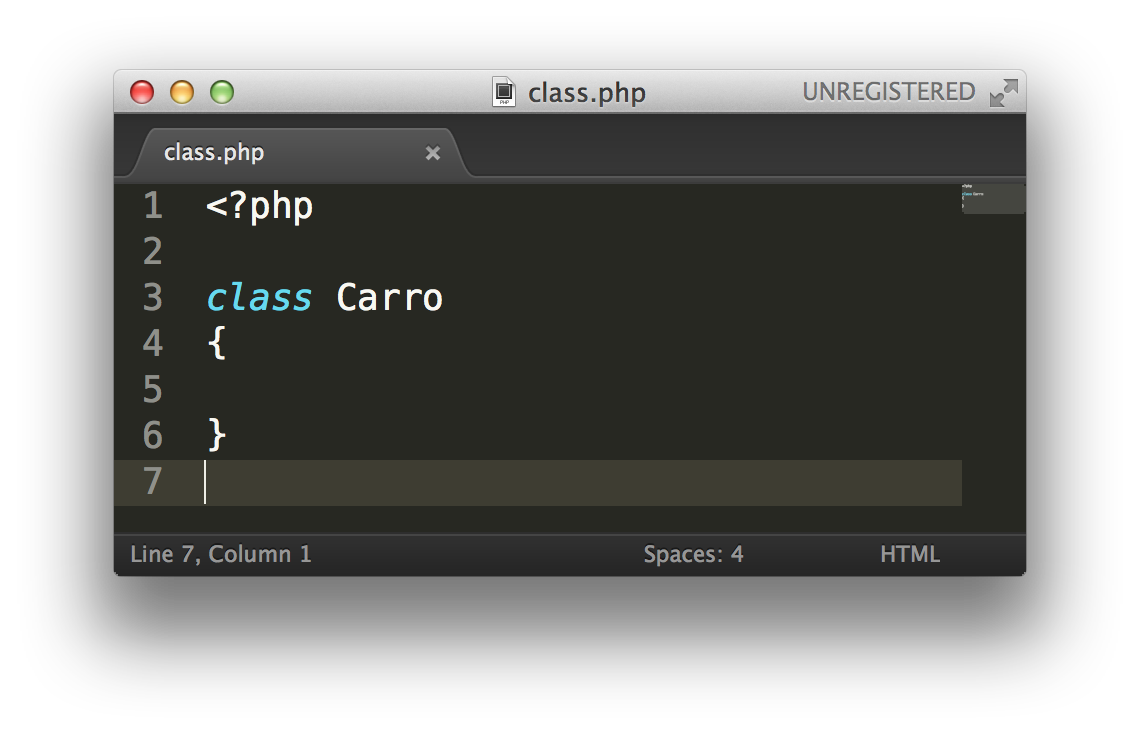
\includegraphics[width=\textwidth]{images/class.png}
	\label{fig:classe}
	\centering
	\footnotesize Fonte: \fonteOAutor
\end{figure}

\FloatBarrier 	% Este comando impede que as imagens 
				% flutuem a partir deste ponto no seu documento

Logo abaixo será apresentada a análise do código exibido na
figura \ref{fig:classe}:

\begin{enumerate}[a)]
    \item \textbf{linha 1:} temos o início da execução de um bloco de código
    PHP;
    \item \textbf{linha 3:} informamos ao interpretador da linguagem PHP que 
    estamos definindo um novo tipo de dados (uma nova estrutura) que será 
    identificada através do nome "Carro";
    \item \textbf{linha 4:} o símbolo \textbf{\{} se refere a abertura de um
    bloco de código, ou seja, informa ao interpretador onde inicia-se a definição de 
    características ou dados (propriedades ou atributos) e ações (métodos). 
    Ambos os conceitos métodos e propriedades veremos ao decorrer deste
    capítulo;
    \item \textbf{linha 6:} o símbolo \textbf{\}} se refere ao fechamento de um
    bloco de código, ou seja, informa ao interpretador onde terminam as
    definições de propriedades e métodos.
\end{enumerate}
\subsection{Objeto}

Um objeto é uma estrutura dinâmica construída com base em uma classe. Sendo que,
com base em uma classe é possível criar vários objetos, cada qual com suas
propriedades \cite{phpProgramandoComOrientacaoAObjetos}.

De forma breve, os objetos são as instâncias de uma classe. Sendo que, as
classes existem somente no código fonte de uma aplicação, enquanto que, as
instâncias de uma classe existem durante a execução de um programa. Portanto,
o software poderá criar vários objetos sob demanda tendo como base um mesmo
modelo \cite{ios7ProgrammingFundamentalsObjectiveCXcodeAndCocoaBasics}. Deste
modo, esses objetos são criados (instanciados) através de métodos construtores
e destruídos (eliminados) através de métodos destrutores em tempo de execução
\cite{umlEC++GuiaPraticoDeDesenvolvimentoOrientadoAObjeto}. Será apresentado no
decorrer deste capítulo como funcionam os métodos construtores e destrutores.

\begin{figure}[h!tb]
	\caption{Criação de um objeto na linguagem PHP}
	\label{fig:objeto}

	\centering
	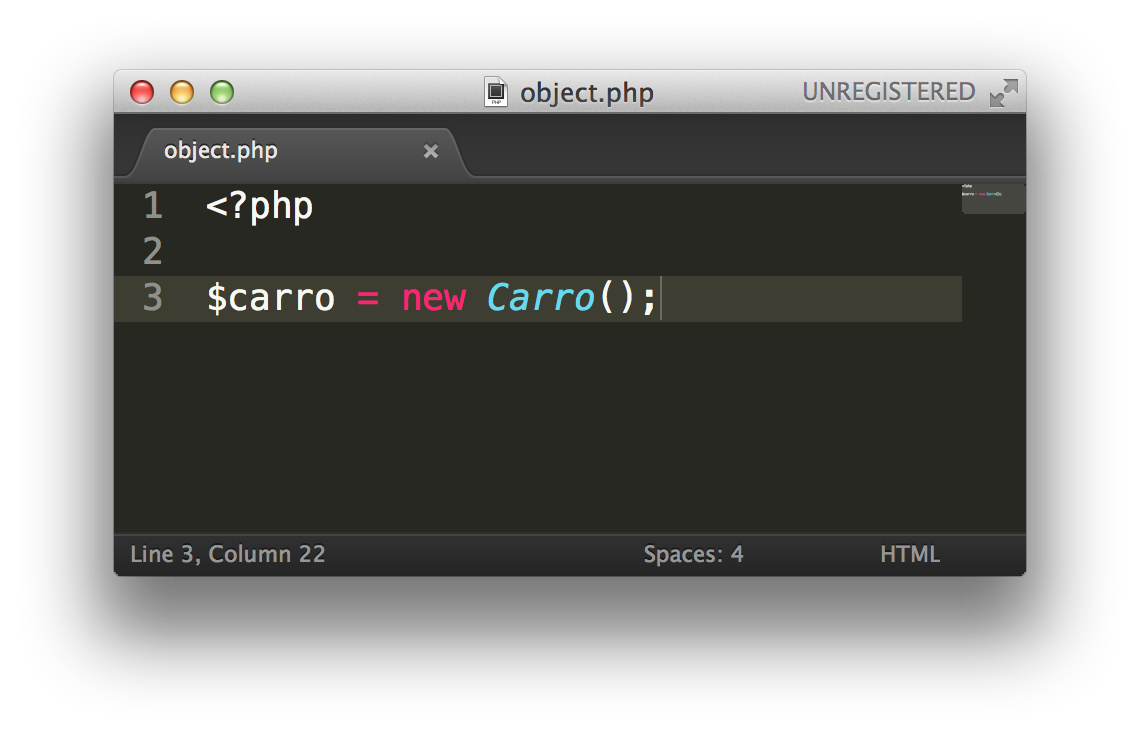
\includegraphics[width=0.65\textwidth]{images/object.png}

	\centering
	\footnotesize Fonte: \fonteOAutor
\end{figure}

\FloatBarrier 	% Este comando impede que as imagens
				% flutuem a partir deste ponto no seu documento

A seguir, será apresentada a análise do código exibido na
Figura \ref{fig:objeto}:

\begin{alineas}
    \item linha 1: tem-se o início da execução de um bloco de código PHP;
    \item linha 3: é definida uma variável chamada \textbf{\$carro};
    chama-se um operador de atribuição da linguagem (representado pelo símbolo
    \textbf{=}) que irá atribuir o valor que está à direita do operador na
    variável que está à esquerda; em seguida é informado um outro operador da
    linguagem (representado pelo símbolo \textbf{new}) que é responsável por
    criar uma referência em memória para o tipo de dados que está sendo
    criado e, por fim, define-se a classe que deverá ser instanciada, que neste
    caso, chama-se Carro. Logo após, o símbolo \textbf{()} representa um método
    construtor (conceito que será apresentado ainda neste capítulo de Orientação
    a Objetos).
    Uma informação importante é que toda instrução da linguagem \acs{PHP} termina
    com o símbolo de ponto-e-vírgula.
\end{alineas}
\subsection{Método}

Segundo \citeonline{php5ConceitosProgramacaoEIntegracaoComBancoDeDados}, um
método pode ser definido como sendo as operações que manipulam os dados de uma
classe, ou seja, definem o que as classes podem e sabem fazer, como por exemplo
acelerar um carro modificando o valor de sua propriedade chamada
\textit{velocidade} para um valor crescente em um determinado espaço de tempo.

Os métodos também podem ser chamados de funções membro \cite{c++ComoProgramar}.

Se comparado a programação estruturada um método pode ser considerado como sendo
uma função que está associada a uma classe \cite{programmingPhp}.

\begin{figure}[h!tb]
	\caption{Criação de um Método utilizando a linguagem PHP}
	\label{fig:metodo}

	\centering
	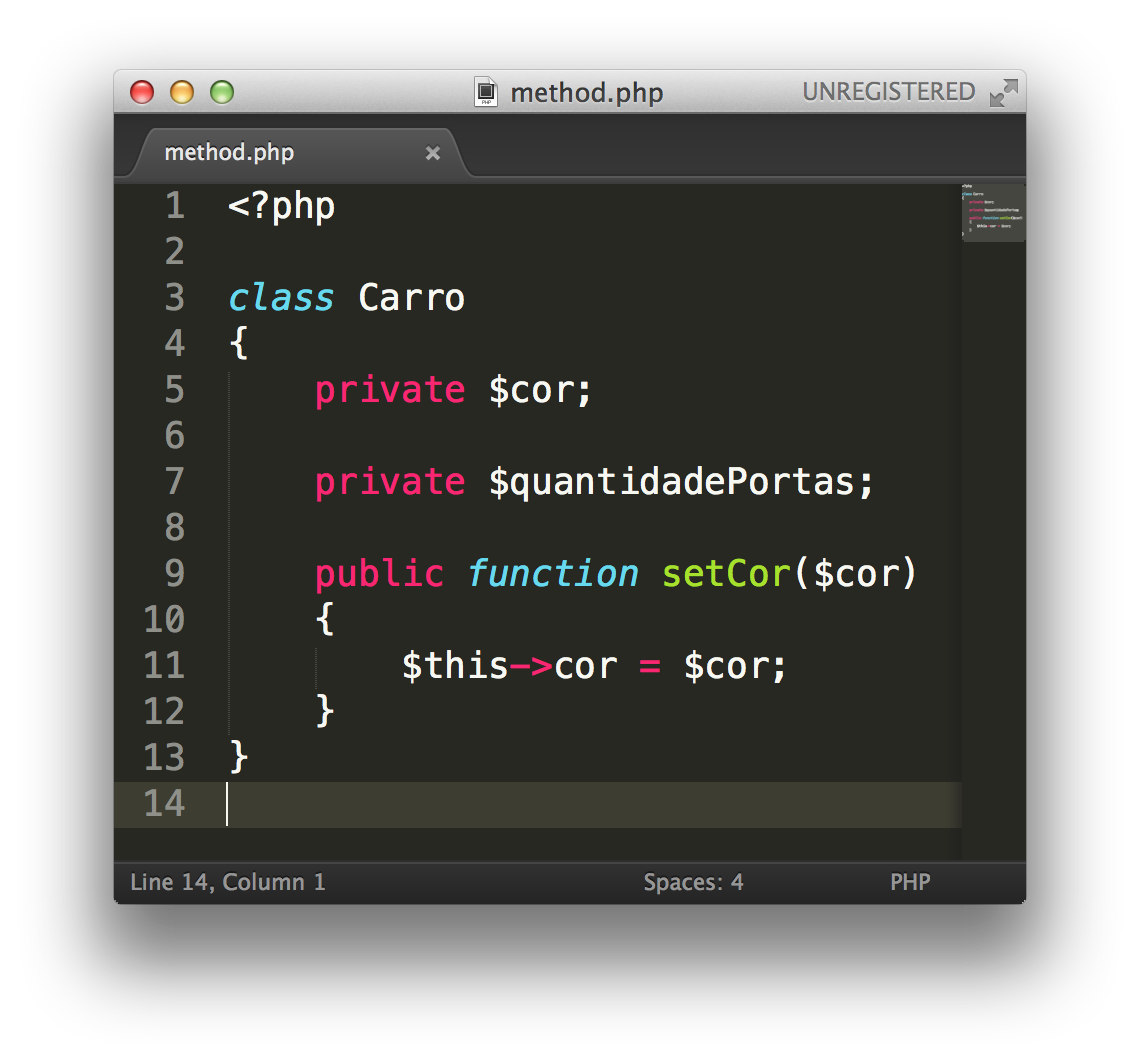
\includegraphics[width=0.68\textwidth]{images/method.png}

	\centering
	\footnotesize Fonte: \fonteOAutor
\end{figure}

\FloatBarrier 	% Este comando impede que as imagens
				% flutuem a partir deste ponto no seu documento

Na sequência, você irá conferir uma explicação referente ao código que foi
apresentado na Figura \ref{fig:metodo}:

\begin{enumerate}[a)]
    \item linha 1: vê-se o início da execução de um bloco de código PHP;
    \item linha 3: define-se uma classe chamada \textit{Carro};
    \item linha 4: informa-se onde inicia o bloco de uma classe;
    \item linha 5 e 7: cria-se duas propriedades para a classe
    \textit{Carro};
    \item linha 9: é solicitado para que o interpretador crie um método
    cuja visibilidade seja pública e define-se que este método será identificado
    pelo nome \textbf{setCor}.
    Além disso, informa-se que este método deve receber um parâmetro (um valor
    que  irá configurar a propriedade de uma classe);
    \item linha 10: define-se onde inicia o bloco cujo escopo
    corresponda ao método \textbf{setCor};
    \item linha 11: utilizou-se uma variável especial chamada
    \textbf{\$this}, esta variável permite acessar qualquer propriedade ou
    método dentro da própria classe ou \textit{superclasse}; depois, usou-se
    o operador de acesso a um objeto (representado pelo símbolo \textbf{->}); em
    seguida, informa-se ao interpretador do \acs{PHP}, a necessidade de
    manipular o valor da propriedade \textit{cor}, sendo que, ela deverá receber o valor
    informado como parâmetro para o método \textbf{setCor};
    \item linha 12: define-se onde termina o bloco que corresponde ao
    método \textbf{setCor};
    \item linha 13: informa-se o encerramento do bloco de uma classe.
\end{enumerate}

Como foi visto o conceito de métodos a seguir será apresentado o conceito de
propriedades.

\subsection{Propriedade}

Assim como a comparação realizada anteriormente, que abordou o que é um método
comparando-o com os conceitos da programação estruturada, seguindo a mesma
analogia, uma propriedade (também conhecida como atributo, variável membro ou ainda variável
de instância) pode ser considerada como os dados que um objeto possuí,
descrevendo desta forma, as características que a ele pertencem
\cite{programmingPhp}.

Sendo assim, os atributos são variáveis que estão definidas dentro de uma
classe, deste modo, geralmente são acessados através de uma interface de acesso,
pois não estão visíveis para que outros objetos manipulem os dados diretamente,
se isto ocorresse, poderia comprometer a segurança da informação e também o
conceito de que cada objeto possuí uma finalidade.

Então, uma propriedade (pensando na classe Carro) poderia ser uma característica
que um carro possuí no mundo real. Portanto, é possível levantar de acordo com
o nosso conhecimento rapidamente os seguintes parâmetros que definem um carro:
cor, quantidade de portas, possuí direção hidráulica, etc.

Na Figura \ref{fig:propriedade}, é apresentada a sintaxe para definição de duas
propriedades (cor e quantidade de portas) da classe Carro implementadas na
linguagem \acs{PHP}.

\begin{figure}[h!tb]
	\caption{Criação de propriedades na linguagem PHP}
	\label{fig:propriedade}

	\centering
	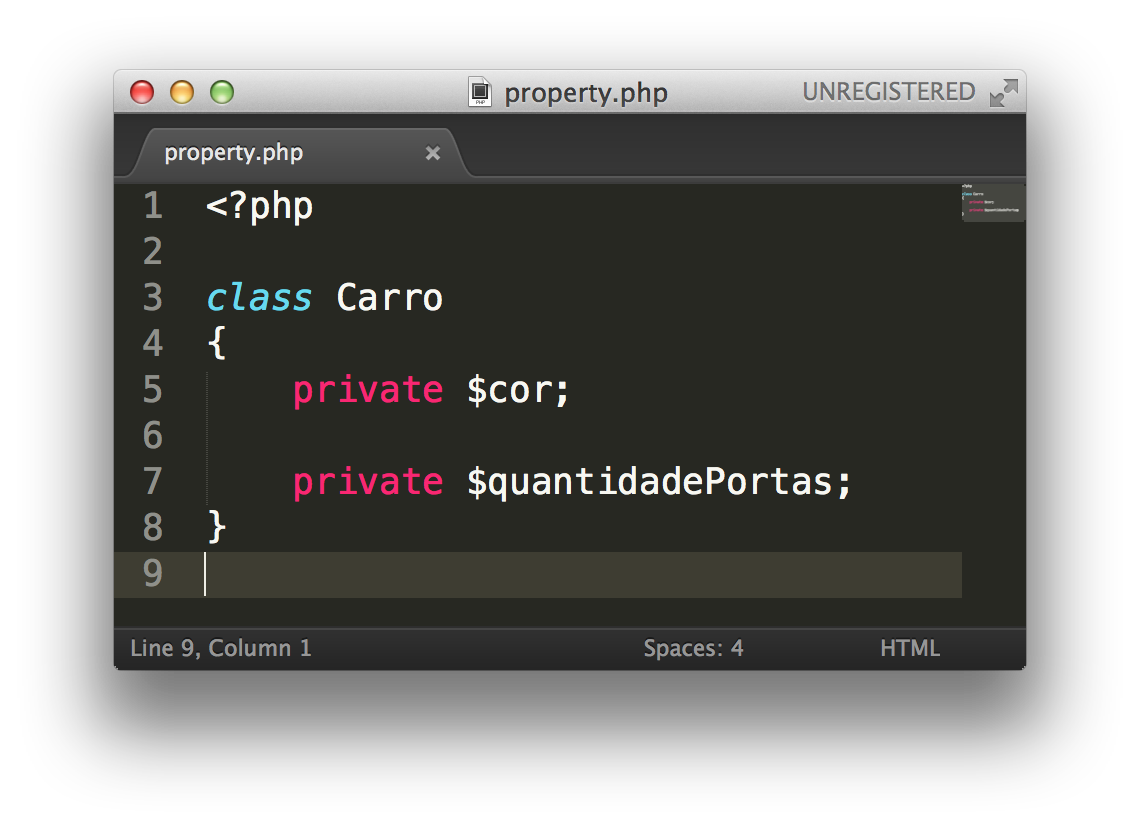
\includegraphics[width=0.75\textwidth]{images/property.png}

	\centering
	\footnotesize Fonte: \fonteOAutor
\end{figure}

\FloatBarrier 	% Este comando impede que as imagens
				% flutuem a partir deste ponto no seu documento

Por conseguinte, abaixo será apresentada a análise das linhas de código
exibidas na Figura \ref{fig:propriedade}:

\begin{alineas}
    \item linha 1: vê-se o início da execução de um bloco de código PHP;
    \item linha 3: define-se uma classe chamada \textit{Carro};
    \item linha 5: utiliza-se uma palavra reservada \textbf{private} que se
    refere a visibilidade da propriedade no contexto de um conjunto de objetos
    (mais detalhes serão apresentadas adiante) e, em seguida, é definido o nome
    de uma variável, que neste caso chama-se \textbf{\$cor};
    \item linha 7: é definida uma segunda propriedade para a classe
    Carro chamada de \textbf{\$quantidadePortas};
    \item linha 8: informa-se onde termina o bloco que compreende a
    classe \textit{Carro}.
\end{alineas}

\subsubsection{Propriedade estática}

Como foi visto anteriormente, as classes são formadas por variáveis de instância
e métodos. Entretanto, as variáveis que forem declaradas com a palavra reservada
\textit{static}, serão compartilhadas por toda a classe. Por conta disto, as
variáveis que assim forem definidas, recebem o nome de variáveis estáticas ou ainda
propriedades estáticas \cite{learningJava}.

Conforme afirma \citeonline{c++ComoProgramar}, a palavra chave \textit{static}
é utilizada quando as informações precisam ser compartilhadas por todas
as instância e não apenas em um único objeto.

Na Figura \ref{fig:propriedadeEstatica} é exibido um exemplo de propriedade
estática utilizando a linguagem \acs{PHP}.

\begin{figure}[h!tb]
	\caption{Propriedade estática definida na linguagem PHP}
	\label{fig:propriedadeEstatica}

	\centering
	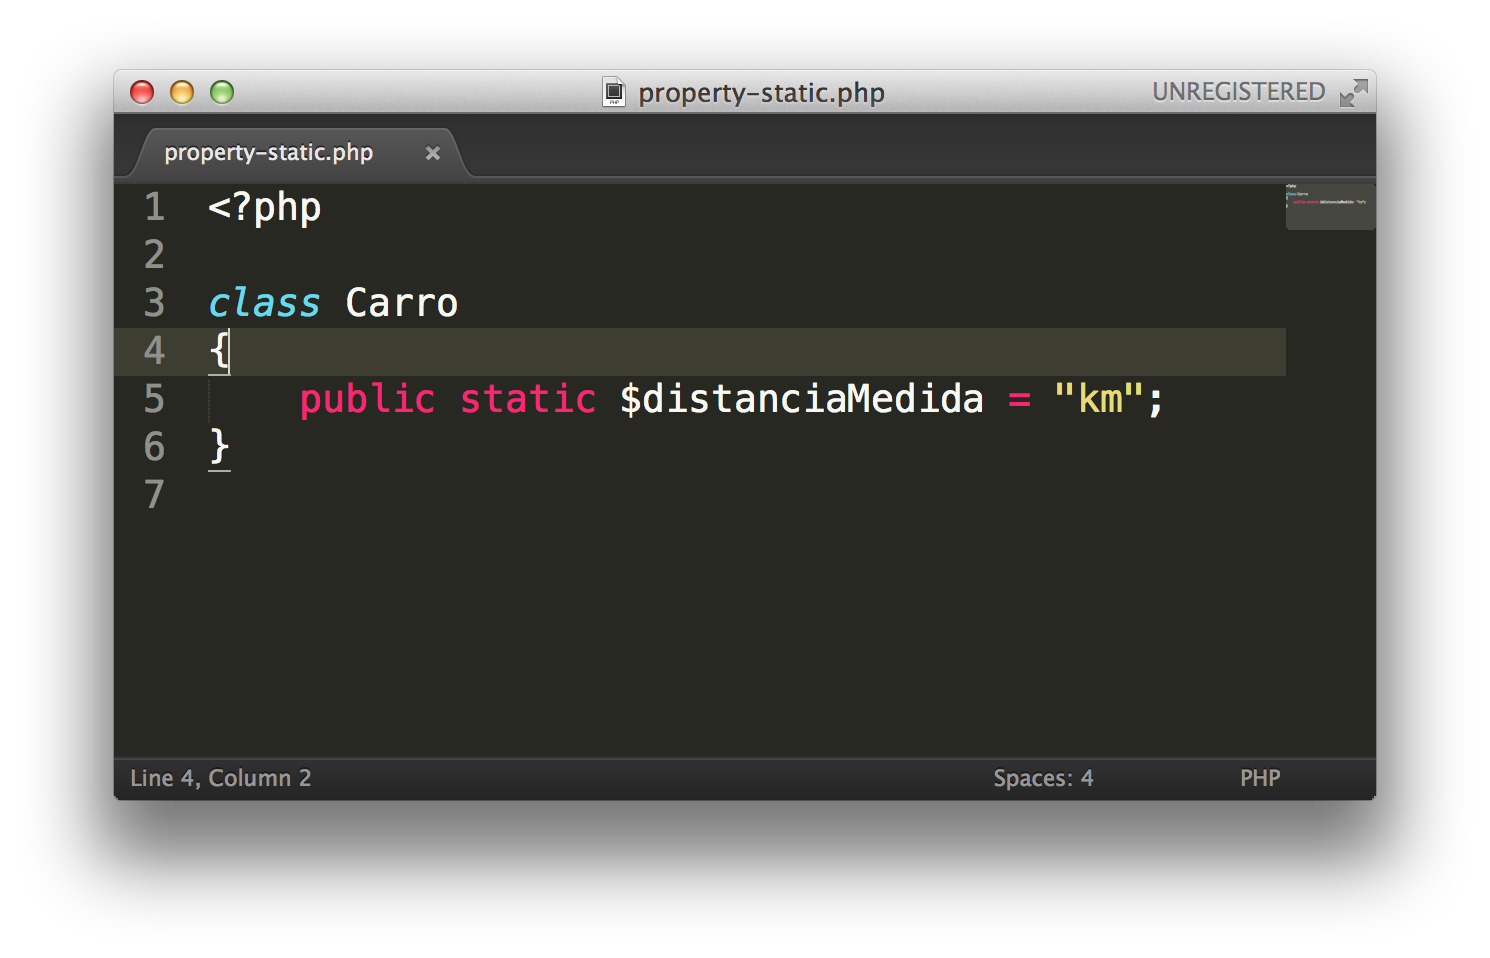
\includegraphics[width=0.82\textwidth]{images/property-static.png}

	\centering
	\footnotesize Fonte: \fonteOAutor
\end{figure}

\FloatBarrier 	% Este comando impede que as imagens
				% flutuem a partir deste ponto no seu documento

A seguir, é apresentado em detalhes as linhas de código exibidas na Figura
\ref{fig:propriedadeEstatica}:

\begin{alineas}
    \item linha 1: vê-se o início da execução de um bloco de código PHP;
    \item linha 5: define-se a propriedade estática que armazenará a unidade de
    medida utilizada por todos os veículos, que neste caso é \textit{km}
    (quilômetros).
\end{alineas}

A seguir será apresentado o conceito que define o que é uma constante e
exibido um exemplo de uso implementado na linguagem \acs{PHP}.

\subsection{Constante}

Assim como as constantes globais utilizadas na linguagem de programação
\acs{PHP} através da função \textit{define}, esta tecnologia também dispõem de
uma maneira que permite definirmos uma constante em uma classe ou em uma
interface. Da mesma maneira que as propriedades estáticas as constantes podem
ser acessadas diretamente de dentro do escopo da classe utilizando-se de um
operador especial denominado \textit{self}, ou ainda, no caso da constante, ser
acessada de fora do escopo da classe através do nome da classe \cite{programmingPhp}.

Quando uma constante de uma classe é definida - da mesma maneira que uma
constante global -  seu valor não poderá ser alterado no decorrer da vida útil
da aplicação. Uma prática comumente utilizada pelos desenvolvedores de software
é definir o nome de uma constante com caixa alta, isto permite que ela seja
identificada rapidamente em um trecho de código. Por conseguinte, uma constante
é um identificador que recebe apenas um valor de inicialização, por conta disto,
seu valor não poderá ser alterado durante a execução do aplicativo.

A seguir na Figura \ref{fig:constante}, é apresentado um exemplo de implementação
de uma constante utilizando a linguagem de programação \acs{PHP}:

\begin{figure}[h!tb]
	\caption{Constante declarada na linguagem PHP}
	\label{fig:constante}

	\centering
	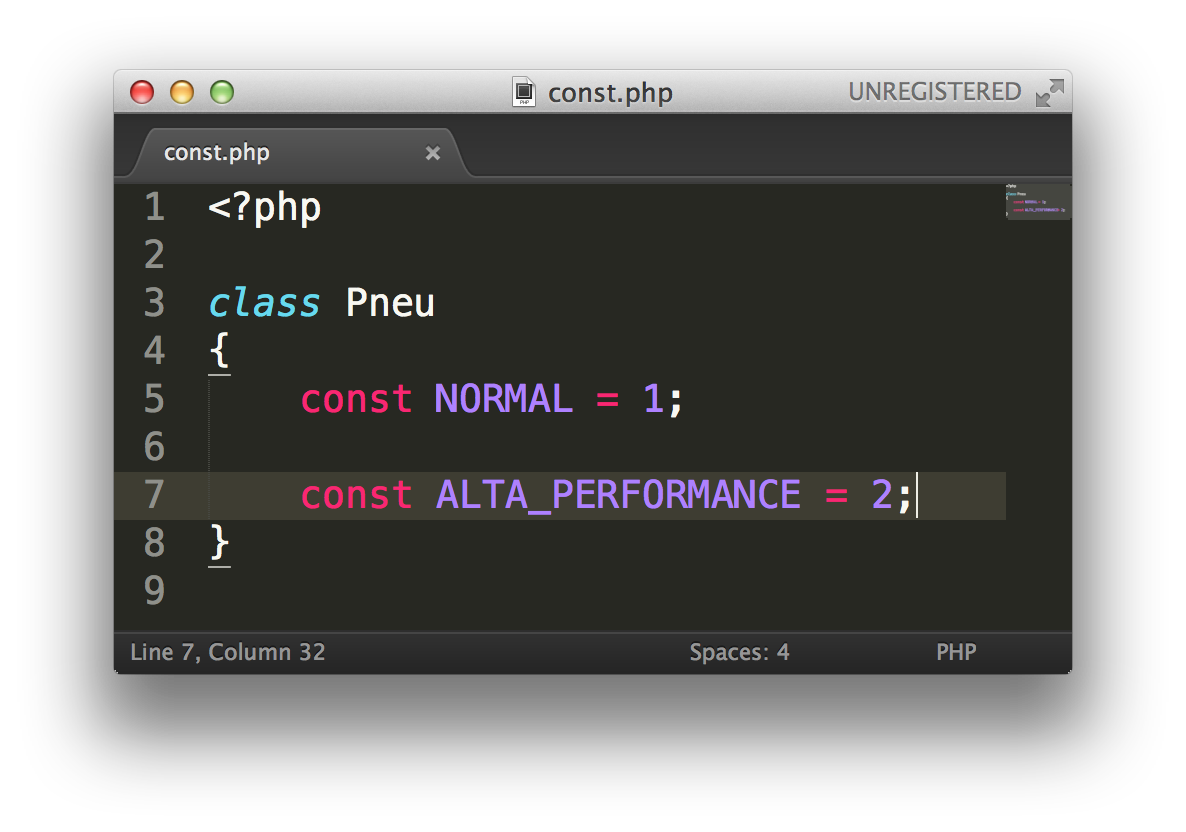
\includegraphics[width=0.75\textwidth]{images/const.png}

	\centering
	\footnotesize Fonte: \fonteOAutor
\end{figure}

\FloatBarrier 	% Este comando impede que as imagens
				% flutuem a partir deste ponto no seu documento

Na sequência, apresenta-se em detalhes as linhas de código exibidas na Figura
\ref{fig:constante}:

\begin{alineas}
    \item linha 1: vê-se o início da execução de um bloco de código PHP;
    \item linha 3: identifica-se a declaração da classe \textit{Pneu};
    \item linha 5: define-se a constante que representa um pneu normal,
    atribuindo a ela o valor numérico 1, que pode ser um código de
    identificação;
    \item linha 7: informa-se outra constante relativa a outro tipo de pneu,
    neste caso, o de alta performance.
\end{alineas}

Logo a seguir, exibe-se o conceito de mensagem que permite que os
objetos se comuniquem entre si.

\subsection{Mensagem}

Um software que foi desenvolvido utilizando os conceitos da orientação a
objetos tem sua execução através da comunicação entre os diversos componentes
de software, estes componentes chamados de objetos trocam mensagens com o
objetivo de realizar uma tarefa, isto se faz necessário porque cada objeto  tem
uma responsabilidade para o qual foi projetado na fase de análise.

Assim sendo, uma mensagem é um pedido para que um objeto execute uma ação
através da chamada de um método, sendo que, este pode alterar o estado de
outros objetos a fim de completar a sua tarefa e, quando ele finalmente termina
a sua execução, geralmente notifica quem solicitou a execução do serviço, ou
seja, retorna algum valor para o objeto que solicitou a operação
\cite{c++ComoProgramar}.

Na Figura \ref{fig:mensagem}, é ilustrado o disparo de uma mensagem na linguagem
\acs{PHP}:

\begin{figure}[h!tb]
	\caption{Chamada de um método utilizando a linguagem PHP}
	\label{fig:mensagem}

	\centering
	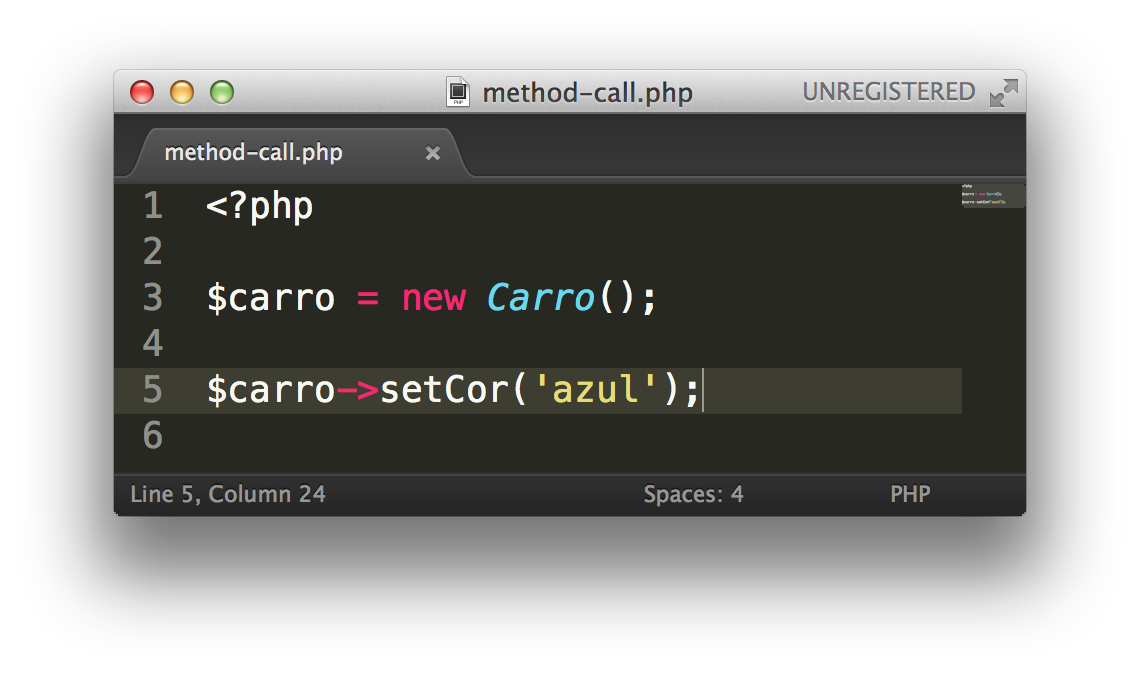
\includegraphics[width=0.6\textwidth]{images/method-call.png}

	\centering
	\footnotesize Fonte: \fonteOAutor
\end{figure}

\FloatBarrier 	% Este comando impede que as imagens
				% flutuem a partir deste ponto no seu documento

A seguir, realiza-se a explicação referente ao código que foi
apresentado na Figura \ref{fig:mensagem}:

\begin{alineas}
    \item linha 1: tem-se o início da execução de um bloco de código
    \acs{PHP};
    \item linha 3: ocorre a criação de um objeto do tipo \textit{Carro};
    \item linha 5: realiza-se a chamada de um método chamado
    \textit{setCor}, sendo que, informa-se um parâmetro para ele, que na
    linguagem \acs{PHP} representa uma \textit{string} (cadeira de caracteres).
    Isto envia uma mensagem para que a classe \textit{Carro} configure
    a propriedade \textit{cor} para receber o valor \textit{azul}.
\end{alineas}

Como foi visto na Figura \ref{fig:mensagem}, o objeto pode invocar um método
público descrito na Classe \textit{Carro} a fim de configurar a cor de um
veículo passando uma mensagem com a cor solicitada.

A seguir, será apresentado o conceito de métodos construtores e como eles podem
colaborar com o desenvolvimento de software inicializando valores de
propriedades.

\section{CONSTRUTOR}

Como vimos anteriormente através de exemplos utilizando linguagem de 
programação PHP, os objetos são criados (instanciados) utilizando-se um 
operador especial, este operador chama-se \textit{new}.

Segundo \citeonline{learningJava}, um construtor é um método especial que tem
como responsabilidade inicializar as propriedades de uma classe. Sendo que, 
diferentemente de outras linguagens, como por exemplo Java que nomeia o  método
construtor com o mesmo nome da classe, a linguagem de script PHP define  que um
método construtor deve chamar-se \textit{\_\_construct}.

Sabendo disto, toda vez que o interpretador encontrar a palavra reservada
\textit{new} este irá executar o método construtor da classe que está sendo 
instanciada.

Caso você defina uma classe e não informe explicitamente um método construtor, a
linguagem em tempo de execução irá inicializar as propriedades com valores nulos.

Além disto, os métodos construtores - da mesma forma que métodos convencionais –
podem aceitar parâmetros de inicialização \cite{learningJava}.

Portanto, os métodos construtores são peças-chave para permitir a configuração 
inicial de um objeto.

Veremos abaixo um exemplo de método construtor utilizando a linguagem PHP:

Uma vez que conhecemos os conceitos de métodos construtores, veremos a seguir  o
conceito de métodos destrutores.
\section{DESTRUTOR}

A linguagem PHP 5, traz consigo o conceito de métodos destrutores de maneira 
similar a outras linguagens orientadas a objeto, como o \textit{Java}. Um método 
destrutor é um método especial, que na linguagem PHP chama-se
\textit{\_\_destruct}, em contrapartida, segundo \citeonline{learningJava}, na
linguagem \textit{Java} o método recebe o nome \textit{finalize}.

Portanto, sempre que um script terminar a sua execução ou quando um objeto for
forçadamente removido, o interpretador irá remover as referências de um objeto 
da memória e o método destrutor será executado.

Enfim, como já conhecemos os conceitos de inicialização e destruição de objetos,
veremos a seguir o conceito de herança.

\subsection{Herança}

Neste capítulo serão definidos os princípios da herança, sendo que, são eles que
permitem que a programação orientada a objetos seja considerada tão poderosa.

Segundo \citeonline{programmingInObjectiveC}, através deste conceito você poderá
construir uma classe com base em uma outra classe já existente e personalizá-la
de acordo com a regra de negócio exigida pela sua aplicação.

Na Figura \ref{fig:heranca}, tem-se a sintaxe da utilização da herança
implementado na linguagem \acs{PHP}:

\begin{figure}[h!tb]
	\caption{Herança na linguagem PHP}
	\label{fig:heranca}

	\centering
	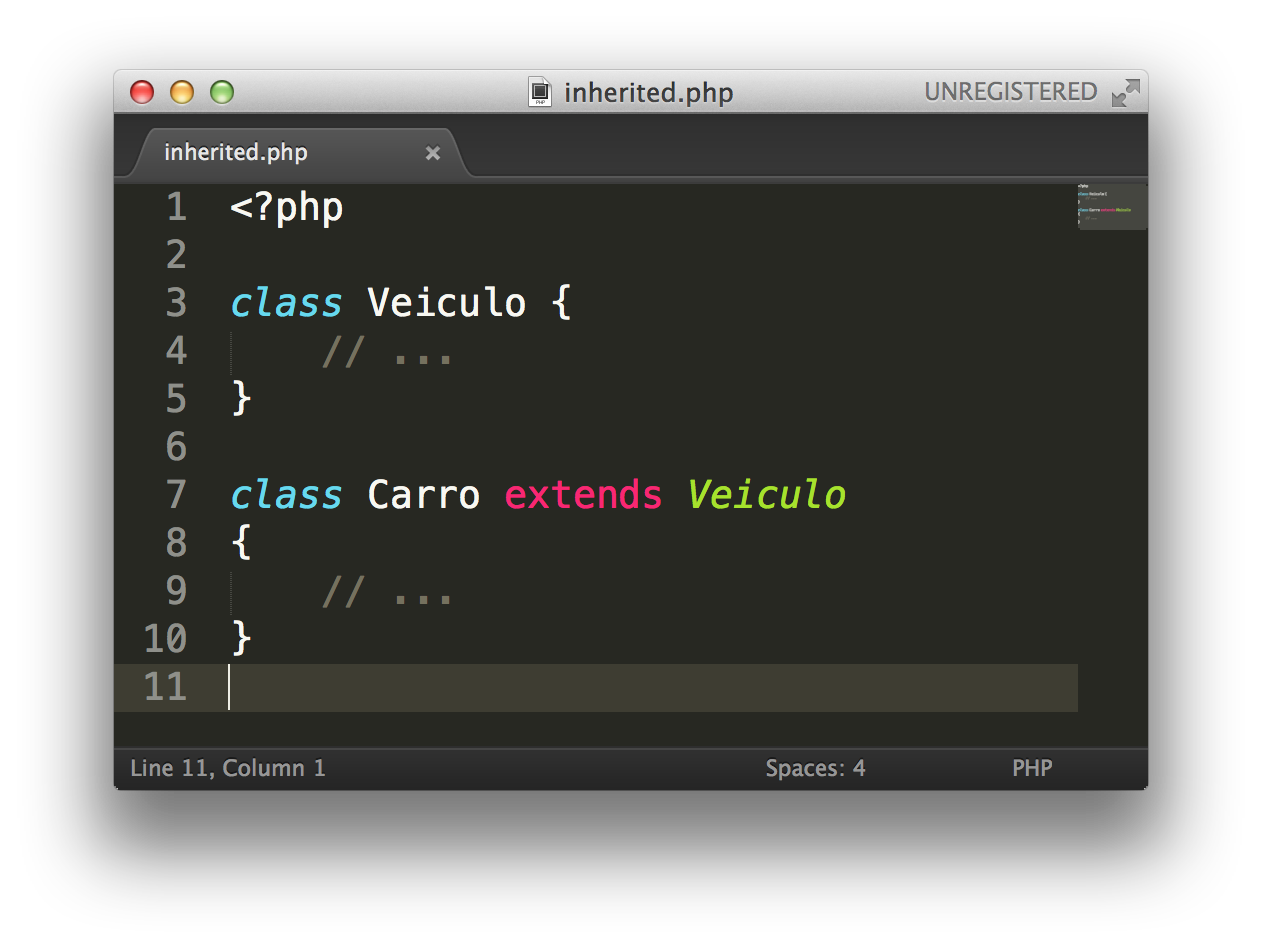
\includegraphics[width=0.75\textwidth]{images/inherited.png}

	\centering
	\footnotesize Fonte: \fonteOAutor
\end{figure}

\FloatBarrier 	% Este comando impede que as imagens
				% flutuem a partir deste ponto no seu documento

A seguir, é apresentado em detalhes as linhas de código exibidas na Figura 
\ref{fig:heranca}:

\begin{enumerate}[a)]
    \item linha 3: definição da classe base \textit{Veiculo};
    \item linha 7: cria-se a classe filha \textit{Carro} com base na classe
    \textit{Veiculo}.
\end{enumerate}

Uma vez definido o conceito de herança, a seguir será abordardado outro conceito
da orientação a objetos, o polimorfismo.

\subsection{Polimorfismo}

Polimorfismo é a capacidade que dois ou mais objetos de uma classe-filha tem  de
responder a mensagens de diferentes formas
\cite{php5ConceitosProgramacaoEIntegracaoComBancoDeDados}.

Ou seja, polimorfismo é a possibilidade que um objeto tem de alterar o
comportamento de um objeto com base em uma classe especialista, sendo assim,
são métodos que fornecem resultados distintos  de acordo com a subclasse
\cite{php5ConceitosProgramacaoEIntegracaoComBancoDeDados}. Desta forma quem
chama o método não precisa distingui-lo.

A seguir, será apresentado a atribuição deste conceito no processo de aceleração
de um veículo. Por conta disto, imagine o exemplo a seguir: dentre os comandos
disponíveis em um veículo, tem-se o acelerador que fornece uma interface
encapsulando a forma de como um motor realiza a aceleração. Agora vamos
supor que deseja-se acelerar dois veículos diferentes, o primeiro veículo
trata-se de um carro popular com motor 1.0, enquanto que, o outro veículo é um
 esportivo, e por conta disto, estamos falando de um carro com motor 2.0. Então,
ambos os veículos possuem a mesma interface de comunicação: o pedal acelerador,
que permite ao condutor se locomover de maneira mais rápida.

Note, que quando o condutor acelerar o carro popular este deverá ter aceleração
mais lenta se comparado ao esportivo, na prática é disto que se trata o polimorfismo.

Voltando-se para o paradigma da orientação a objetos seria possível existir uma
classe generalista chamada \textit{Carro} que seria responsável em definir um
meio padronizado para realizar a aceleração de um veículo. E, com base nesta
classe, criar duas outras classes especialistas, sendo que, poderiam ser
nomeadas como: \textit{CarroPopular} e \textit{CarroEsportivo}.

Na Figura \ref{fig:polimorfismo} será apresentada a implementação destes conceitos
utilizando a linguagem de programação \acs{PHP}.

\begin{figure}[h!tb]
	\caption{Polimorfismo com implementação na linguagem PHP}
	\label{fig:polimorfismo}

	\centering
	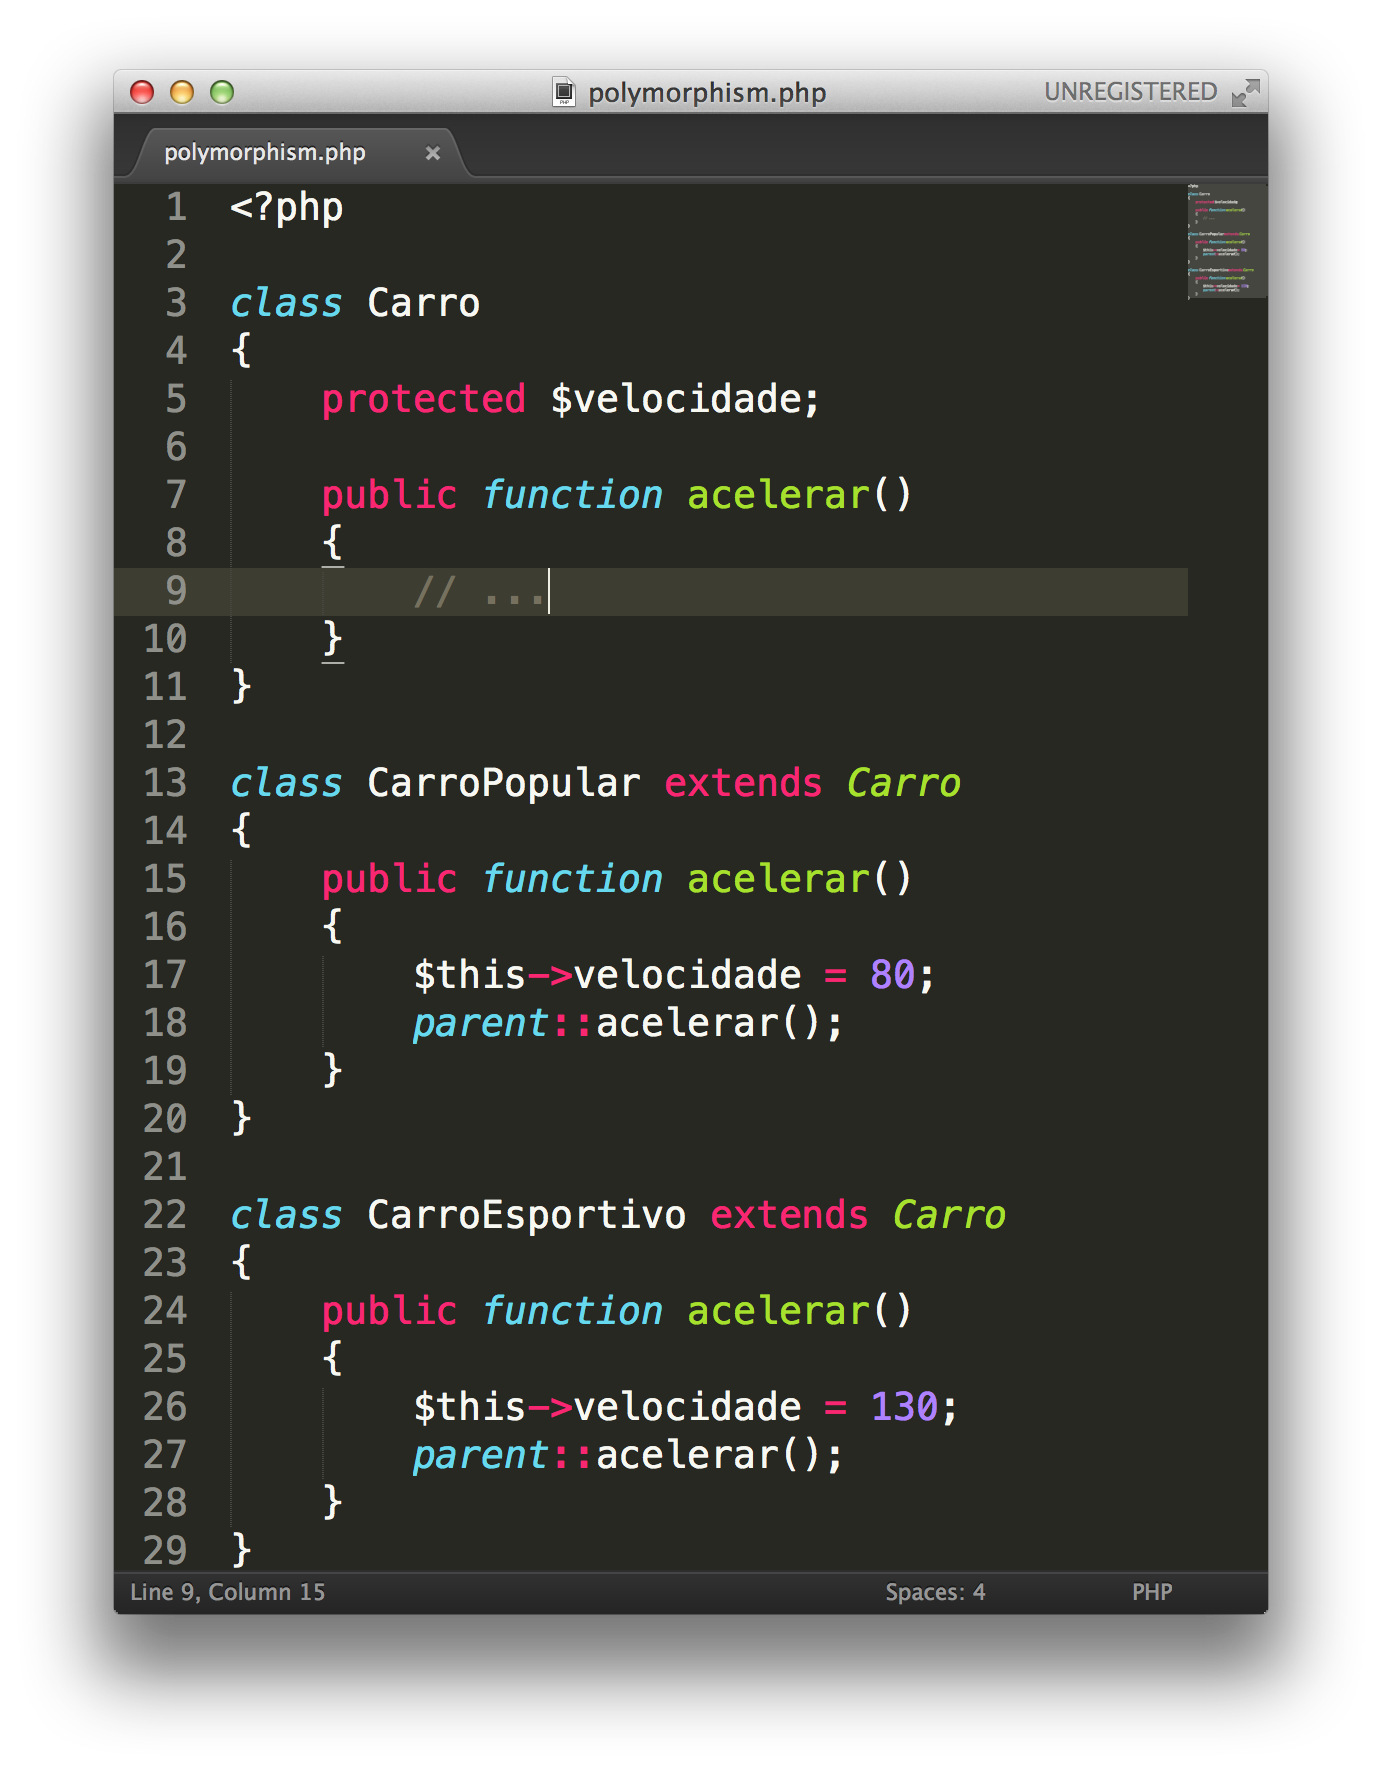
\includegraphics[width=0.75\textwidth]{images/polymorphism.png}

	\centering
	\footnotesize Fonte: \fonteOAutor
\end{figure}

\FloatBarrier 	% Este comando impede que as imagens
				% flutuem a partir deste ponto no seu documento

A seguir, é apresentado em detalhes as linhas de código exibidas na Figura
\ref{fig:polimorfismo}:

\begin{alineas}
    \item linha 3: define-se a existência da classe \textit{Carro};
    \item linha 4: tem-se a declaração do método \textit{acelerar} que trata de
    uma forma padrão de acelerar qualquer veículo;
    \item linha 13: define-se a classe \textit{CarroPopular}, sendo que, ela
    herda todas as características e funcionalidades da classe \textit{Carro};
    \item linha 15: reescreve-se o método \textit{acelerar} que foi definido na
    classe \textit{Carro}, pois, um carro popular acelera neste caso a uma
    velocidade de oitenta quilômetros por hora;
    \item linha 22: define-se a classe \textit{CarroEsportivo}, que, da mesma
    maneira que a classe \textit{CarroPopular} herda as propriedades e métodos
    que foram definidos na classe pai \textit{Carro};
    \item linha 24: redefine-se o método \textit{acelerar}, pois, um carro
    esportivo acelera a uma velocidade constante de cento e trinta quilômetros
    por hora (neste caso).
\end{alineas}

Conforme foi visto neste capítulo, ambos os veículos aceleram, entretanto o
carro esportivo tem um desempenho melhor do que o carro popular, entretanto, a
modelagem permite reusar a classe carro e definir apenas as características
pertinentes a ambos os veículos, sendo assim, os objetos que chamarem esta
classe não entendem como a implementação acontece, mas realmente aceleram de
maneira correspondente ao tipo de veículo.

A seguir será apresentado o conceito de encapsulamento, que permite esconder do
escopo público os dados sensíveis, tais como as propriedades de uma classe.

\subsection{Encapsulamento}

Até então quando foi realizada a criação de propriedades para a nossa
classe, elas foram definidas com a visibilidade: privada, do inglês,
\textit{private}. Sendo que, sempre que definirmos as propriedades e métodos em 
uma classe deve-se informar qual a  sua visibilidade. Por conseguinte, existem 
três visibilidades, são elas: privada, protegida e pública. Segundo 
\citeonline{javaComoProgramar}, os conceitos de visibilidade também são
chamados de modificadores de acesso.

A visibilidade privada, do inglês \textit{private}, permite acesso somente
dentro do escopo da classe que definiu a propriedade ou método. Enquanto que, a
visibilidade protegida, do inglês \textit{protected}, permite que todas as
classes  que herdam propriedades ou métodos tenham acesso dentro do escopo da classe filha.
Em contrapartida, a visibilidade pública, do inglês \textit{public}, permite que
qualquer objeto que tenha instanciado um objeto da classe que definiu uma propriedade ou
método possa invoca-lo no caso do método, ou modificar o seu estado no caso de
uma propriedade \cite{learningJava}.

Sendo assim, por questões de segurança da aplicação é interessante fornecer
interfaces para manipulação dos estados de um objeto. Por conta disto,  sempre
que definirmos uma propriedade em uma classe será utilizadar a visibilidade
privada, caso essa classe não implemente conceitos de herança posteriormente, 
ou então, com visibilidade protegida afim de permitir que as classes
especialistas  herdem as suas definições. E, é justamente este o conceito de 
encapsulamento, realizar o ocultamento dos dados ou informações \cite{javaComoProgramar}.

Mas, para que um cliente de um objeto – todos os objetos que estão fora do
escopo da classe -  possam modificar os estados das propriedades, são criados
métodos especialistas conhecidos como: métodos \textit{getters} e \textit{setters}.

\subsubsection{Métodos getters e setters}

São métodos responsáveis por modificar e recuperar os estados de uma variável
membro de uma classe permitindo que esta função membro esteja exposta a todo o
escopo da aplicação.

No caso do método configurar, do inglês \textit{set}, ele permite que os
clientes de um objeto configurem novos valores para uma propriedade, realizando
antecipadamente uma ação para validar a entrada de dados por exemplo.

Em contrapartida, existe o método obter, do inglês \textit{get}, que recupera o
valor de uma propriedade, sendo que, este método poderia realizar por exemplo uma
formatação adequada de uma propriedade.

Sendo que, o nome desses métodos (por conta de uma convenção de atribuição de
nomes) recebe o prefixo \textit{set} ou \textit{get} seguido do nome da
propriedade, tendo esta a sua primeira letra em caixa alta \cite{javaComoProgramar}.
\subsection{Exceções}

A linguagem de programação \acs{PHP} 5, introduz o conceito de exceções, e isto traz
uma grande vantagem se comparada a manipulação de erros das versões anteriores
da tecnologia, além disto, pode-se também encontrar similaridades nos
conceitos aplicados ao \acs{PHP}, caso tenha-se conhecimento de outras
linguagens, tais como: \textit{Java} e \textit{C++} \cite{phpObjectsPatternsAndPractice}.

Uma exceção indica que ocorreu uma condição não esperada ou um erro, sendo que,
isto geralmente acontece por conta de um erro de processamento, como por
exemplo: uma atribuição ou leitura de valores incorretos ou obrigatórios em
variáveis locais e propriedades durante a execuçao de um método \cite{learningJava}.

Segundo \citeonline{phpObjectsPatternsAndPractice} uma exceção é um objeto
especial instanciado a partir da classe \textit{Exception}, ou a partir de uma
classe especialista, portanto, estes objetos são projetados para criar e
reportar informações de erro.

Sendo assim, se comparado a forma tradicional de manipulação de erros, as
exceções são uma forma elegante de manipulá-los e tratá-los dentro de uma
aplicação, de acordo com o que foi visto no capítulo que
tratava sobre herança, pode-se extender as funcionalidas da classe
\textit{Exception}, personalizando os seus dados e o seu comportamento \cite{phpMasterWriteCuttingEdgeCode}.

Conforme afirma \citeonline{phpMasterWriteCuttingEdgeCode}, um objeto da classe
\textit{Exception}, irá conter informações referente ao erro que ocorreu, dentre
estas informações estão:

\begin{alineas}
    \item o nome do arquivo;
    \item a linha em que ocorreu o problema;
    \item uma mensagem;
    \item e, opcionalmente, um código de erro.
\end{alineas}

No Quadro \ref{tab:excecao} são apresentados os métodos da classe
\textit{Exception} presente na linguagem de programação \acs{PHP}.

% Esta tabela está na p.52] da referencia: phpObjectsPatternsAndPractice
\begin{table}[h!tb]
	\centering
	\setlength{\belowcaptionskip}{9pt}
	\caption{Métodos públicos da classe \textit{Exception}}
	\begin{tabular}{| l | p{0.7\textwidth} |}

		\hline
		\textbf{Método}
		& \textbf{Descrição} \\
		\hline

        \textit{getMessage()}
        & Recupera uma \textit{string} que foi enviada
        para o construtor.

        \\ \cline{1-2}
        \textit{getCode()}
        & Recupera o código de erro.
        \\ \cline{1-2}

        \textit{getFile()}
        & Recupera o arquivo em que a exceção foi lançada.
        \\ \cline{1-2}

        \textit{getLine()}
        & Recupera o número da linha em que a exceção ocorreu.
        \\ \cline{1-2}

        \textit{getPrevious()}
        & Recupera um objeto de uma exceção.
        \\ \cline{1-2}

        \textit{getTrace()}
        & Recupera um \textit{array} multimensional contendo as chamadas de
        métodos, incluindo: funções membro, classes, arquivos e argumentos. \\
        \cline{1-2}

        \textit{getTraceAsString()}
        & Recupera os dados de \textit{getTrace()} no formato de uma
        \textit{string}.
        \\ \cline{1-2}

        \textit{\_\_toString()}
        & Método mágico executado automaticamente quando um objeto é exibido em
        tela como uma \textit{string}. Sendo assim, retorna uma \textit{string}
        descrevendo os detalhes da exceção.
        \\
        \hline
	\end{tabular}
	\newline
	\newline
	\label{tab:excecao}
	\begin{footnotesize}
		Fonte: adaptado de \cite[p.53]{phpObjectsPatternsAndPractice}
	\end{footnotesize}
\end{table}

\FloatBarrier 	% Este comando impede que as imagens
				% flutuem a partir deste ponto no seu documento


Na sequência, será apresentado na Figura \ref{fig:excecao} a manipulação de um
erro de processamento utilizando a classe \textit{Exception}, onde, para que
um erro de processamento não deixasse de interromper a execução, poderia haver
uma cor inexistente e quando esta fosse informada um erro seria gerado e 
manipulado através de um bloco \textit{try/catch}.

\begin{figure}[h!tb]
	\caption{Classe \textit{Exception} da linguagem PHP}
	\label{fig:excecao}

	\centering
	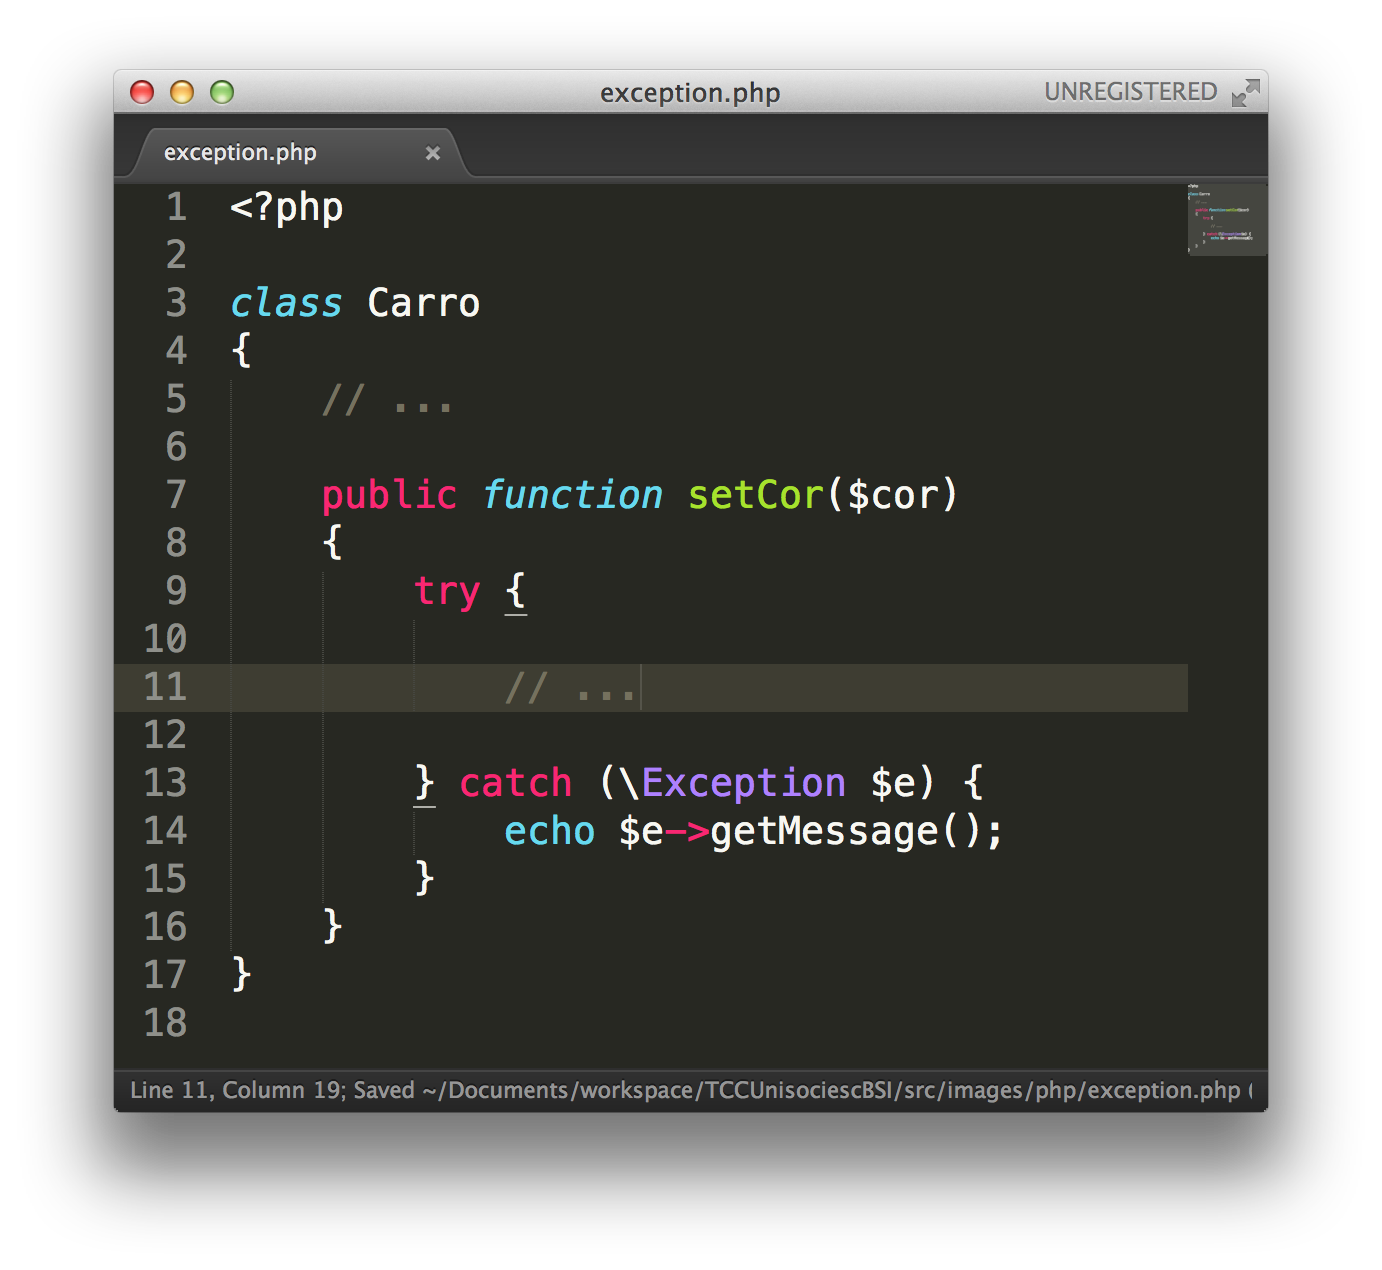
\includegraphics[width=0.75\textwidth]{images/exception.png}

	\centering
	\footnotesize Fonte: \fonteOAutor
\end{figure}

\FloatBarrier 	% Este comando impede que as imagens
				% flutuem a partir deste ponto no seu documento

A seguir, é apresentado em detalhes as linhas de código exibidas na Figura
\ref{fig:excecao}:

\begin{alineas}
    \item linha 7: define-se um método chamado \textit{setCor};
    \item linha 9: utiliza-se a palavra reservada \textbf{try} informando ao
    \acs{PHP} que o que estiver entre os delimitadores deste bloco pode não
    ocorrer de forma esperada, ou seja, tente realizar este procedimento;
    \item linha 13: caso ocorra algum problema na execução do \textit{script}
    definido na linha 11, o \acs{PHP} irá tratar o erro atribuindo-o a variável
    \textbf{\$e};
    \item linha 14: mostra uma mensagem descritiva com relação ao erro que acaba
    de ocorrer.
\end{alineas}

Em seguida, será apresentado o conceito de interfaces, que permitem definir
contratos de implementação entre as classes, por conseguinte, estas classes
devem cumprir com todas as especificações definidas no contrato.

\subsection{Interface}

As interfaces fornecem uma maneira de definir contratos entre diferentes
classes, portanto, uma interface pode definir: a assinatura de métodos e
valores armazenados através de constantes. Por conta disto, qualquer classe  que
quiser seguir os padrões definidos pela interface deverá assinar um contrato,
ou seja, deverá implementar a assinatura dos métodos da mesma maneira como  fora
definido na interface \cite{programmingPhp}.

Além disto, permite abstrair recursos em sistemas e facilitar a
injeção de dependências, além de garantir a extensibilidade e padronização do
projeto, ou seja, é possível definir que um objeto irá receber como argumento de
um método construtor uma interface, sendo que, é permitido passar como parâmetro
qualquer classe que implemente a interface. Agora, na Figura
\ref{fig:interface}, é apresentado um exemplo referente a definição de uma 
interface utilizando a linguagem \acs{PHP}.

\begin{figure}[h!tb]
	\caption{Interface implementada na linguagem PHP}
	\label{fig:interface}

	\centering
	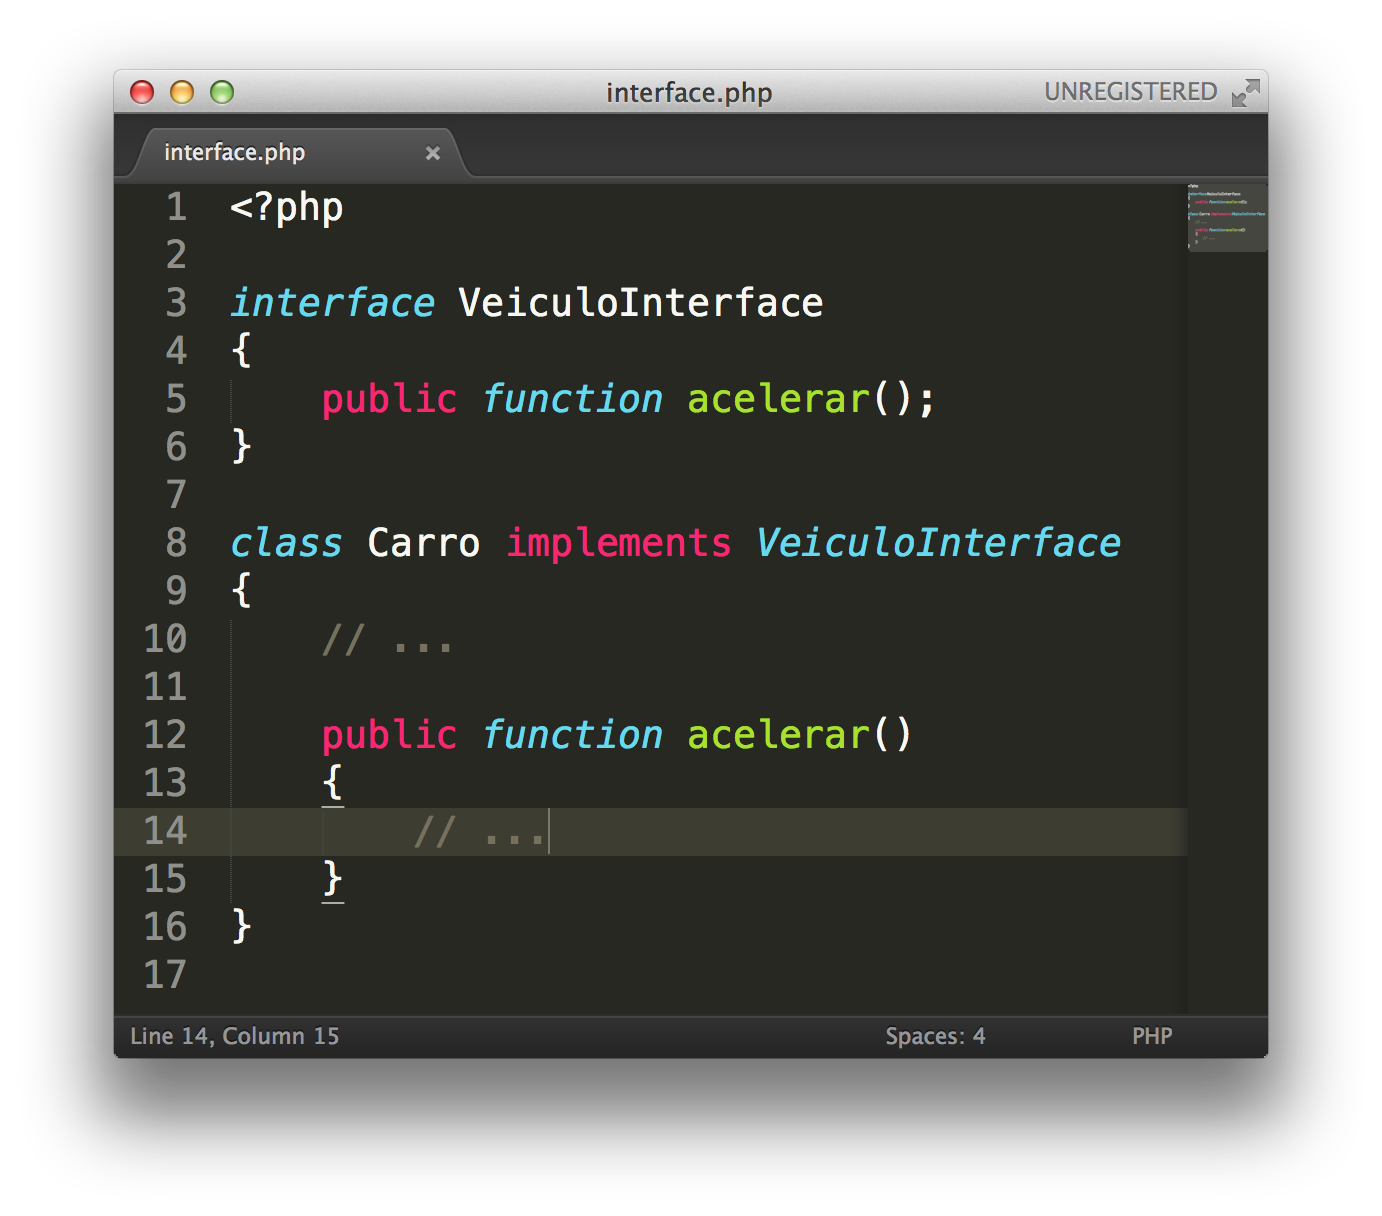
\includegraphics[width=0.75\textwidth]{images/interface.png}

	\centering
	\footnotesize Fonte: \fonteOAutor
\end{figure}

\FloatBarrier 	% Este comando impede que as imagens
				% flutuem a partir deste ponto no seu documento

Abaixo, será apresentado em detalhes as linhas de código exibidas na Figura
\ref{fig:interface}:

\begin{alineas}
    \item linha 3: define-se uma interface nomeada como
    \textit{VeiculoInterface};
    \item linha 5: define-se a assinatura de um método, no qual, todas as
    classes que decidirem assinar um contrato com a interface deverão definir um
    método com a mesma assinatura;
    \item linha 8: implementa-se uma classe chamada \textit{Carro}, sendo que,
    ela assina um contrato com a interface \textit{VeiculoInterface}, por conta
    da palavra chave \textbf{implements};
    \item linha 12: define-se o método que foi solicitado pela interface.
\end{alineas}

Com isto, finaliza-se o capítulo que trata sobre os conceitos de orientação a
objetos com exemplos de implementação na linguagem \acs{PHP}, na sequência será
apresentado o capítulo que tratará sobre banco de dados.

\section{PACOTE}

\textit{Pacote\ldots}
	
	\section{BANCO DE DADOS}

Antes de abordar o banco de dados \acs{MySQL} e o \acs{PostgreSQL} - ambos
bancos livres bastante populares no mercado - é necessário compreender
conceitualmente o que é um banco ou base de dados.
 
Segundo \citeonline{theDefinitiveGuideToMySQL5} um banco de dados pode ser uma
lista de registros que são manipulados por um programa de computador, por
exemplo o \acs{Excel}, ou ainda, pode ser também os arquivos de armazenamento
de uma empresa de telecomunicações referente as várias chamadas que ocorreram
diariamente, além disto, alguns bancos de dados são utilizados por apenas um
usuário, enquanto que outros são acessados por vários usuários
simultaneamente, por conseguinte, uma base pode ocupar poucos ou muitos
kilobytes do dispositivo de armazenamento.

Sendo assim, a palavra \textit{banco de dados} é utilizada para referenciar os
dados reais, o software gerenciador do banco (como por exemplo: \acs{MySQL} e 
\acs{PostgreSQL}), um cliente de conexão ao banco (são exemplos: um script
\acs{PHP} ou um programa escrito em C++), sendo assim, é comum que quando as 
pessoas falem sobre o assunto gerem confusão \cite{theDefinitiveGuideToMySQL5}.

Portanto, conforme afirma \citeonline{phpMySQLForDummies}, o termo banco de
dados, do inglês \textit{database}, se refere a um arquivo ou um grupo de
arquivos contendo dados, sendo que, esses dados são acessados por programas 
chamados de \ac{DBMS}. Quase todos os \acs{DBMS} são \ac{RDBMS}, nos quais
os dados são organizados e armazenados em tabelas relacionais.

Os termos \acs{DBMS} e \acs{RDBMS} também são definidos respectivamente como
\ac{SGBD} e \ac{SGBDR}.

\subsection{MySQL}

De acordo com \citeonline{integrandoPHP5ComMySQL}, \acs{MySQL} é um
\acs{RDBMS},  que utiliza a linguagem \ac{SQL} para manipular os seus registros, 
sendo que, é altamente utilizado em aplicações para a internet e, por
conseguinte,  seu código fonte é aberto, tendo destaque em características
como: velocidade, escalabilidade e confiabilidade, por conta disto, é adotado
pelo departamento de \ac{TI}, desenvolvedores e vendedores de software.

\subsection{PostgreSQL}

Assim como o \acs{MySQL}, o \acs{PostgreSQL} é um \acs{RDBMS} também de
código livre e seu antepassado ficou conhecido como Ingres, sendo que, surgiu na
universidade da Califórnia, em Berkeley
\cite{postgreSQLIntroductionAndConcepts}.

Por conseguinte, possui alguns recursos de bancos empresariais, tais como: a
possibilidade de criar funções agregadas e também a replicação de
\textit{streaming},  certamente, estes recursos raramente são encontrados em 
plataformas livres, mas, são comumente encontrados em bancos comerciais, como:
\textit{SQL Server} e \textit{IBM DB2} e, além destas vantagens, ele pode 
superar bases comerciais  em algumas cargas de trabalho 
\cite{postgreSQLUpAndRunning}.

	\section{DESENVOLVIMENTO FRONT-END}

Geralmente quando desenvolvemos para a web, temos profissionais especialistas em
duas áreas da construção de uma aplicação, são eles: o \textit{frontend} e o
\textit{backend} \cite{artigoAvaliacaoEReducaoDoTempoDeRespostaDeSistemasWeb}.

Segundo \citeonline{artigoAvaliacaoEReducaoDoTempoDeRespostaDeSistemasWeb}, é no
\textit{frontend} que tecnologias como: a \ac{HTML}, as \ac{CSS}, o \ac{JS}
e o conteúdo multimídia são desenvolvidos.

Sendo assim, falaremos neste capítulo sobre essas tecnologias.

\subsection{HTML}

Segundo \citeonline{htmlCSSTheGoodParts} na construção de uma aplicação web ou
um website, uma das tarefas mais importantes é a criação de links entre os
documentos, possibilitando assim a navegação, o \acs{HTML} permite criarmos
estes documentos descrevendo o conteúdo que os usuários acessam ao explorar a web.

Ao acessar um website, o \acs{HTML} informa ao navegador como o seu documento
foi estruturado: qual o título do documento, se existem parágrafos, se existe
algum texto enfatizado, quais são os botões de navegação. Sendo assim, o
navegador renderiza o documento, ou seja, faz a intepretação dos
comandos e exibe para o usuário o resultado final, que neste caso, é a página
web \cite{headFirstHTMLWithCSSAndXHTML}.

Entretanto, o \acs{HTML} não trata a forma como os elementos estão dispostos em
tela e para isto existe uma outra tecnologia responsável por manipular os
elementos visuais, trabalhando de forma integrada ao \acs{HTML}:
o \acs{CSS}, que será apresentado a seguir.

\subsection{CSS}

O \ac{CSS}, do inglês \textit{Cascading Style Sheets}, é uma ferramenta
que webdesiners e também desenvolvedores utilizam em conjunto com o \ac{HTML}
para a construção de websites, onde, o \acs{CSS} proporciona que \ac{browser}
controle os aspectos visuais da página, como por exemplo: o posicionamento de elementos,
estilos de texto, cores, imagens e muito mais, além disto, existem algumas
técnicas avançadas que permitem aos autores a construção de layouts voltados a
dispositivos móveis \cite{beginningCSSCascadingStyleSheetsForWebDesign}.

Sendo assim, o \acs{CSS} permite transformar a apresentação de um ou vários
documentos \acs{HTML}, a seguir será apresentado outro recurso que permite
dinamismo em páginas \acs{HTML}: o \acl{JS}.

\subsection{Javascript}

Segundo \citeonline{javascriptAndJQueryTheMissingManual}, \acl{JS} (\acs{JS}) é
uma linguagem de programação interpretada que permite que um documento \acs{HTML} 
que é estático receba interatividade, animações e efeitos visuais dinâmicos.

A seguir, será apresentada uma das principais bibliotecas disponíveis  para esta
linguagem: o \textit{jQuery}.

\subsubsection{Jquery}

Conforme afirma \citeonline{jQueryABibliotecaDoProgramadorJavaScript}, 
\textit{jQuery} é uma poderosa biblioteca \acl{JS} de código aberto, que foi
concebida com o objetivo de simplificar a interatividade em páginas web, seu 
criador John Resig apresentou o conceito de "\textit{write less, do more}", ou
seja, "escreva menos, faça mais", no qual em um pequeno trecho de código fonte 
utilizando a biblioteca \textit{jQuery}, é possível realizar um procedimento que
teria muito mais linhas de código, para que fosse obtido o mesmo resultado em um
\textit{script} implementado em \acs{JS} sem o uso desta biblioteca.

Sendo assim a biblioteca (\textit{library}) \textit{jQuery} foi construída
utilizando a linguagem de programação \acl{JS}, ou seja, ela não é uma nova 
linguagem de programação \cite{beginningJQuery}.

Portanto, a \textit{library} \textit{jQuery} tem a intenção de tornar a
programação mais fácil e divertida, sendo considerada como um programa complexo
que simplifica tarefas cotidianas com uso de seletores \acs{CSS} e resolve
problemas de compatibilidade com vários navegadores 
\cite{javascriptAndJQueryTheMissingManual}.

\subsection{Twitter Bootstrap}

Segundo \cite{jumpStartResponsiveWebDesign}, o \acs{Twitter Bootstrap}  é uma
das mais famosas bibliotecas de componentes responsivos na web de código fonte
aberto.

De maneira breve, o \textit{framework} permite que desenvolvedores possam criar
projetos web de maneira mais rápida e padronizada, além de permitir que
profissionais que não conheçam profundamente a linguagem de estilização 
\acs{CSS} desenvolvam interfaces agradáveis, sendo que, possuí uma manual 
extensivo que aborda exemplos de implementação, além disto, permite atingir
todos os dispositivos com uso de layouts responsivos e pode ser usado com
pré-processadodores tais como: \ac{LESS} e \ac{SASS}.

	
	% --------------------------------------------------------------------------
	
	\newpage
	
	\chapter{GERENCIAMENTO DE DEPENDENCIAS}
	\section{BOWER}
	\section{COMPOSER}
	
	\chapter{SERVIDORES WEB}
	Para permitir que um usuário acesse um documento web, precisamos disponibilizar
	em um servidor. %ver imagem em headFirstHtmlAndCSS:40
	\section{APACHE}
	\section{NGINX}
	
	\chapter{FRAMEWORK}
	\section{Symfony 2}
	\section{Zend 2}
	
	% --------------------------------------------------------------------------
	
	\bibliography{ref}
	\bibliographystyle{abnt-alf} 
	
\end{document}